\begin{figure*}[t]
	\centering
	\addtolength{\tabcolsep}{-3.5pt}
	\begin{tabular}{cccc}
		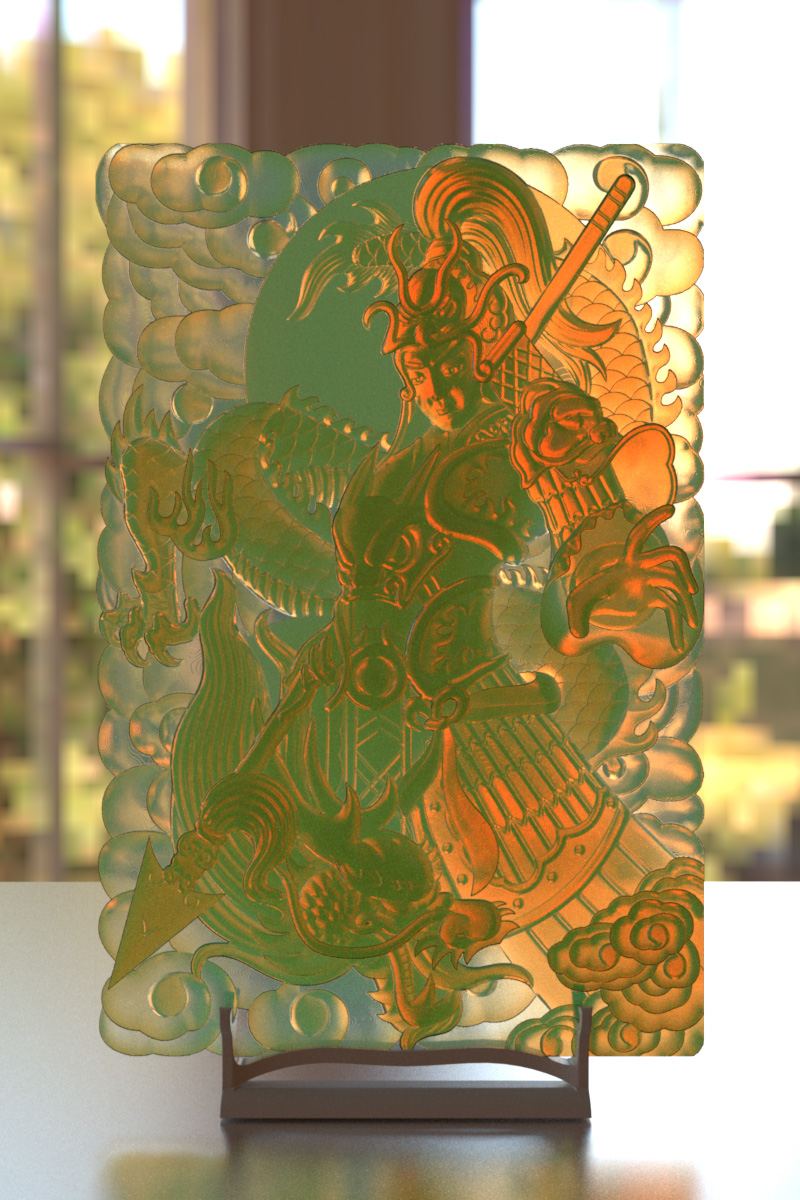
\includegraphics[width=0.24\textwidth]{results/zhaoyun_bg1_1.jpg} &
		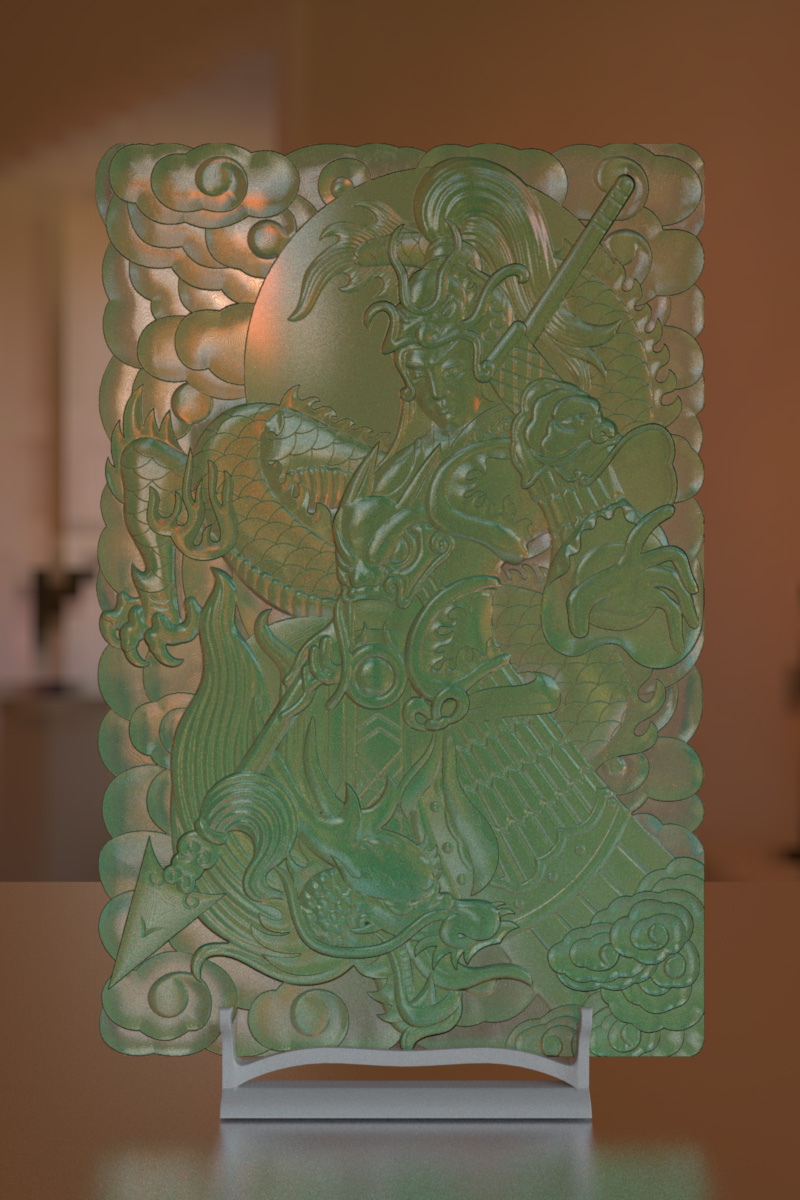
\includegraphics[width=0.24\textwidth]{results/zhaoyun_bg1_2.jpg} &
		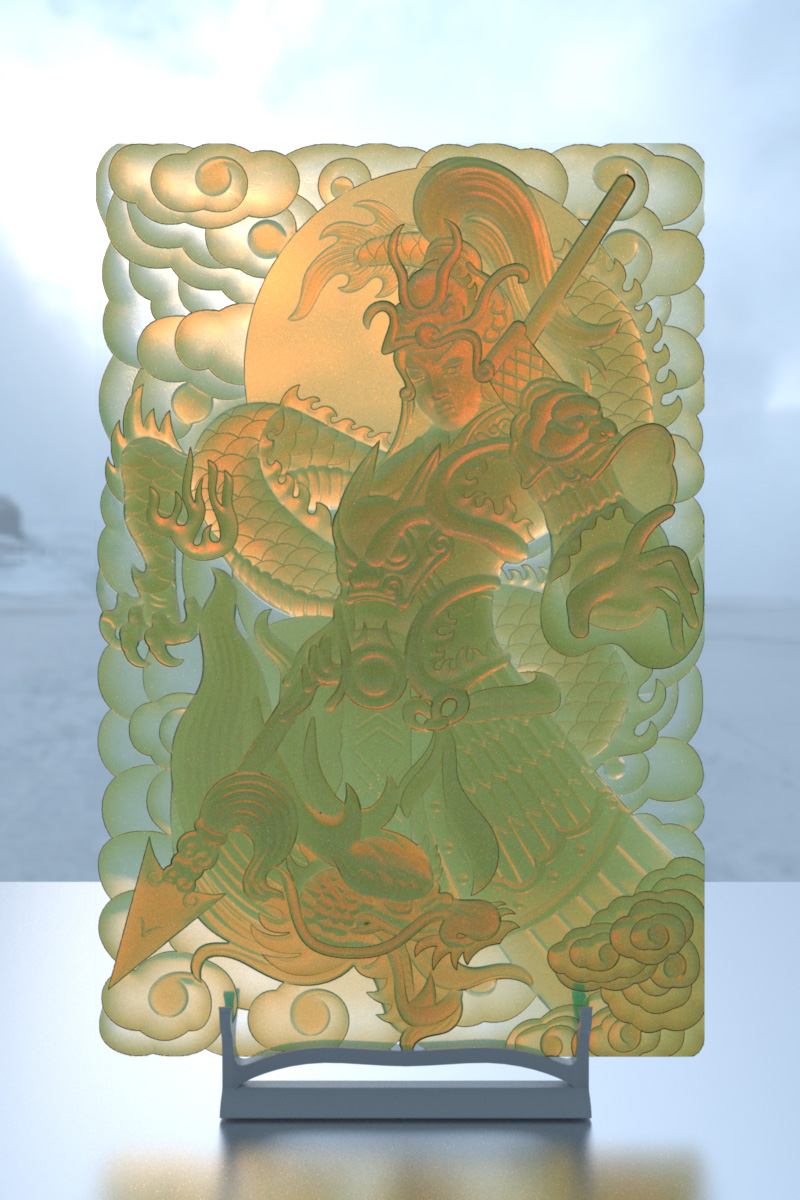
\includegraphics[width=0.24\textwidth]{results/zhaoyun_bg2_1.jpg} &
		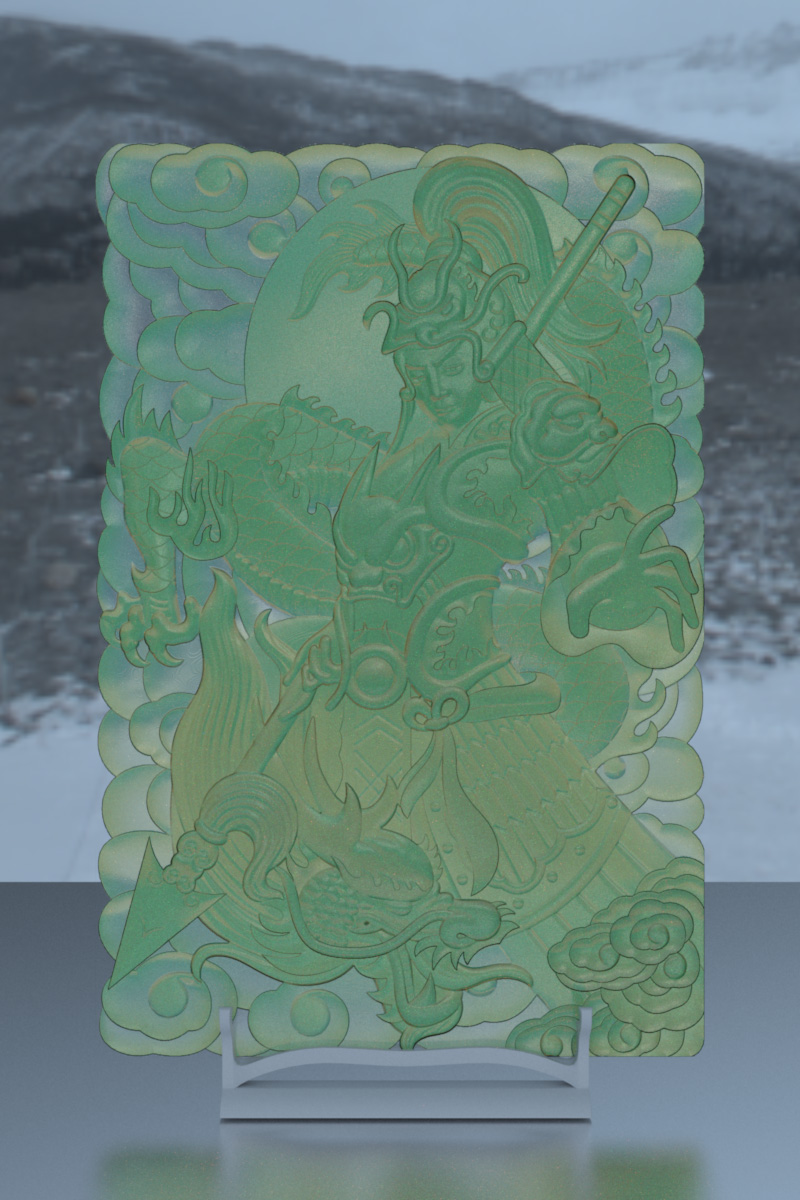
\includegraphics[width=0.24\textwidth]{results/zhaoyun_bg2_2.jpg}\\
		Back-lit & Front-lit & Back-lit & Front-lit
		\\[5pt]
		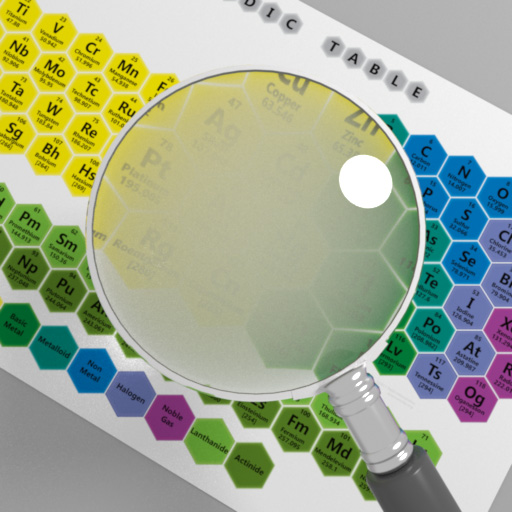
\includegraphics[width=0.24\textwidth]{results/magnify_g9.jpg} &
		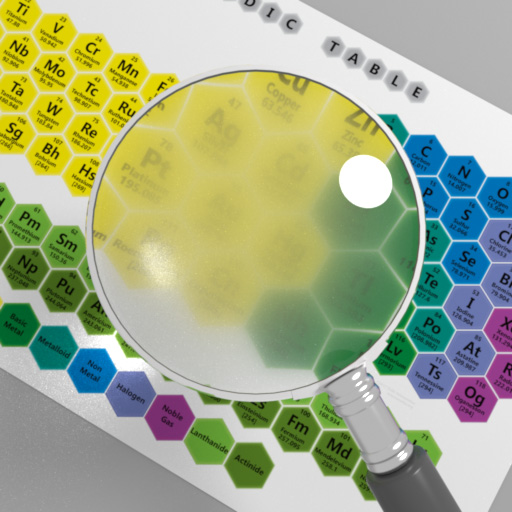
\includegraphics[width=0.24\textwidth]{results/magnify_g99.jpg} &
		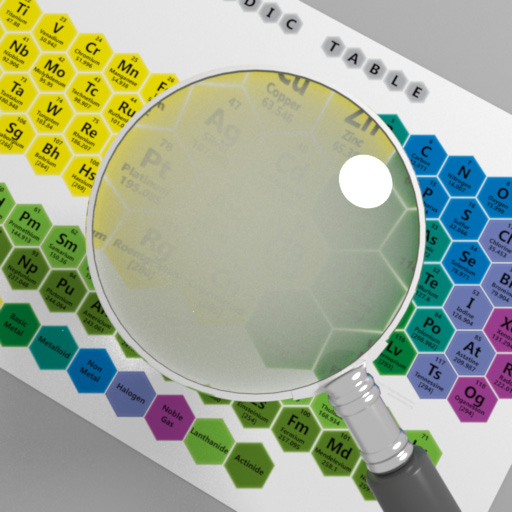
\includegraphics[width=0.24\textwidth]{results/magnify_vmf10.jpg} &
		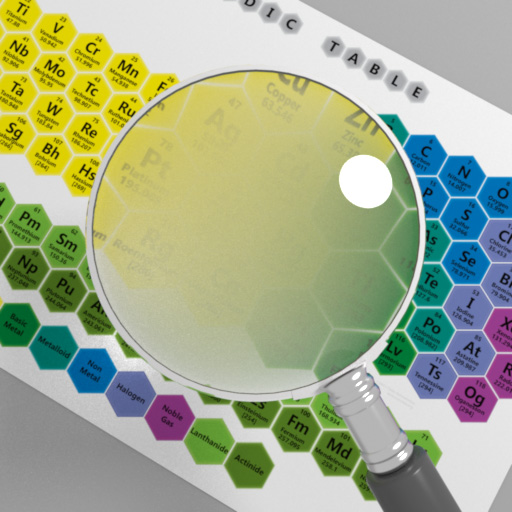
\includegraphics[width=0.24\textwidth]{results/magnify_vmf100.jpg}\\
		HG ($g = 0.9$) & HG ($g = 0.99$) & vMF ($\kappa = 10$) & vMF ($\kappa = 100$)
	\end{tabular}
	%\caption{albedo:0.2,0.95,0.8; $\sigma_t$:1.2,6,12}
	\caption{\label{fig:result_transmit}
		\textbf{Reflection and transmission:}
		Our BSDF models are capable of accurately capturing not only reflection but also transmission from thin layers. \textbf{Top:} A flat surface rendered with our layered BSDF under varying illuminations. This model involves dielectric interfaces with spatially varying roughnesses, normal maps, and thickness. The optical densities (mean free paths) are spectrally varying, which results in subtle color variations across the surface. Note that the color (albedo) is not varying. \textbf{Bottom:} A flat surface with a layered BSDF of spatially varying thickness (which captures the shape of real convex lens). A range of spatially varying and physically plausible blurring effects can be achieved by varying phase functions.
	}
\end{figure*}